\documentclass[aspectratio=169, 11pt]{beamer}

% ===================== PACKAGES =====================
\usepackage{lmodern}
\usepackage[T1]{fontenc}
\usepackage[utf8]{inputenc}
\usepackage{graphicx}
\usepackage{booktabs}
\usepackage{xcolor}
\usepackage{amsmath}
\usepackage{tabularx}
\usepackage{array}
\usepackage{colortbl}

% ===================== COLORS (matching MPSIF report aesthetic) =====================
\definecolor{inertiapurple}{HTML}{5D4E8C}
\definecolor{inertiablue}{HTML}{5B7BC9}
\definecolor{inertiagreen}{HTML}{3FA47D}
\definecolor{inertiared}{HTML}{C84B4B}
\definecolor{inertiamuted}{HTML}{9A9A9A}
\definecolor{lightpurple}{HTML}{EFEAF5}

% ===================== BEAMER THEME =====================
\usetheme{default}
\usecolortheme{default}
\setbeamersize{text margin left=14mm, text margin right=14mm}
\setbeamertemplate{navigation symbols}{}
\setbeamertemplate{headline}{}

\setbeamercolor{frametitle}{fg=inertiapurple, bg=white}
\setbeamerfont{frametitle}{series=\bfseries, size=\Large}
\setbeamertemplate{frametitle}{%
  \vspace{10pt}\hspace{-2pt}\insertframetitle\vspace{-8pt}\\[2pt]
  {\color{inertiapurple}\rule{\textwidth}{0.4pt}}%
}
\setbeamercolor{title}{fg=inertiapurple}
\setbeamercolor{structure}{fg=inertiapurple}
\setbeamercolor{alerted text}{fg=inertiapurple}

\setbeamertemplate{footline}{%
  \leavevmode%
  \hbox{\begin{beamercolorbox}[wd=\paperwidth, ht=3ex, dp=1.5ex,
        leftskip=14mm, rightskip=14mm]{footerline}%
  \hspace*{0pt}\hfill{\tiny\color{gray}\insertframenumber\,/\,\inserttotalframenumber}%
  \end{beamercolorbox}}%
}

\setbeamertemplate{itemize item}{\color{inertiapurple}\footnotesize$\blacksquare$}
\setbeamertemplate{itemize subitem}{\color{inertiablue}\scriptsize$\bullet$}
\setbeamerfont{itemize/enumerate body}{size=\normalsize}

\newcommand{\fundname}{\textsc{Inertia v2}}
\newcommand{\emphp}[1]{{\color{inertiapurple}\textbf{#1}}}
\newcommand{\emphb}[1]{{\color{inertiablue}\textbf{#1}}}
\newcommand{\emphr}[1]{{\color{inertiared}\textbf{#1}}}
\newcommand{\emphg}[1]{{\color{inertiagreen}\textbf{#1}}}

% ===================== DOCUMENT =====================
\begin{document}

% ============================================================
% SLIDE 1: TITLE
% ============================================================
\begin{frame}[plain]
  \vspace{0.6cm}
  \begin{center}
    {\Huge\bfseries\color{inertiapurple} Inertia v2}\\[8pt]
    {\large\itshape Factor Regime Detection for the MPSIF Systematic Sub-Fund}\\[24pt]
    {\color{inertiapurple}\rule{0.45\textwidth}{0.5pt}}\\[18pt]
    {\large Will Wu \,\textbullet\, Kathy Yang}\\[6pt]
    {\normalsize UG54 Data Driven Investing\, \textbullet\, Spring 2026}\\[3pt]
    {\small\color{inertiablue} Topic: Timing Strategies; Factor Investing; Machine Learning}\\[28pt]
    \begin{minipage}{0.78\textwidth}
      \centering\itshape
      Three regime-detection methods, an ensemble that fails, and a hybrid
      defensive overlay that lifts MPSIF's synthetic Sharpe from \textbf{0.80}
      to \textbf{0.88} while cutting max drawdown by 7 points.
    \end{minipage}
  \end{center}
\end{frame}

% ============================================================
% SLIDE 2: THE QUESTION
% ============================================================
\begin{frame}{The question we are answering}
  \vspace{20pt}
  \begin{center}
  \begin{minipage}{0.85\textwidth}
    \begin{itemize}
      \item The MPSIF Systematic Sub-Fund holds 50 stocks chosen from a momentum, growth, and value blend. It is exposed to all five Fama-French factors.
      \item \emphp{Factor premia are time-varying.} Value lost money in the 2010s. Momentum crashed in 2009 and 2022. Quality has cycled.
      \item \emphb{Research question:} can we detect regime changes in major Fama-French factors and use those signals to make MPSIF a better fund?
      \item \emphg{Class connections:} factor models, dynamic mean-variance, regime-switching, regularized regression, gradient boosting, paired bootstrap.
    \end{itemize}
  \end{minipage}
  \end{center}
\end{frame}

% ============================================================
% SLIDE 3: TIME-VARYING FACTOR PREMIA (motivation)
% ============================================================
\begin{frame}{Factor premia are not constant}
  \vspace{-4pt}
  \begin{center}
    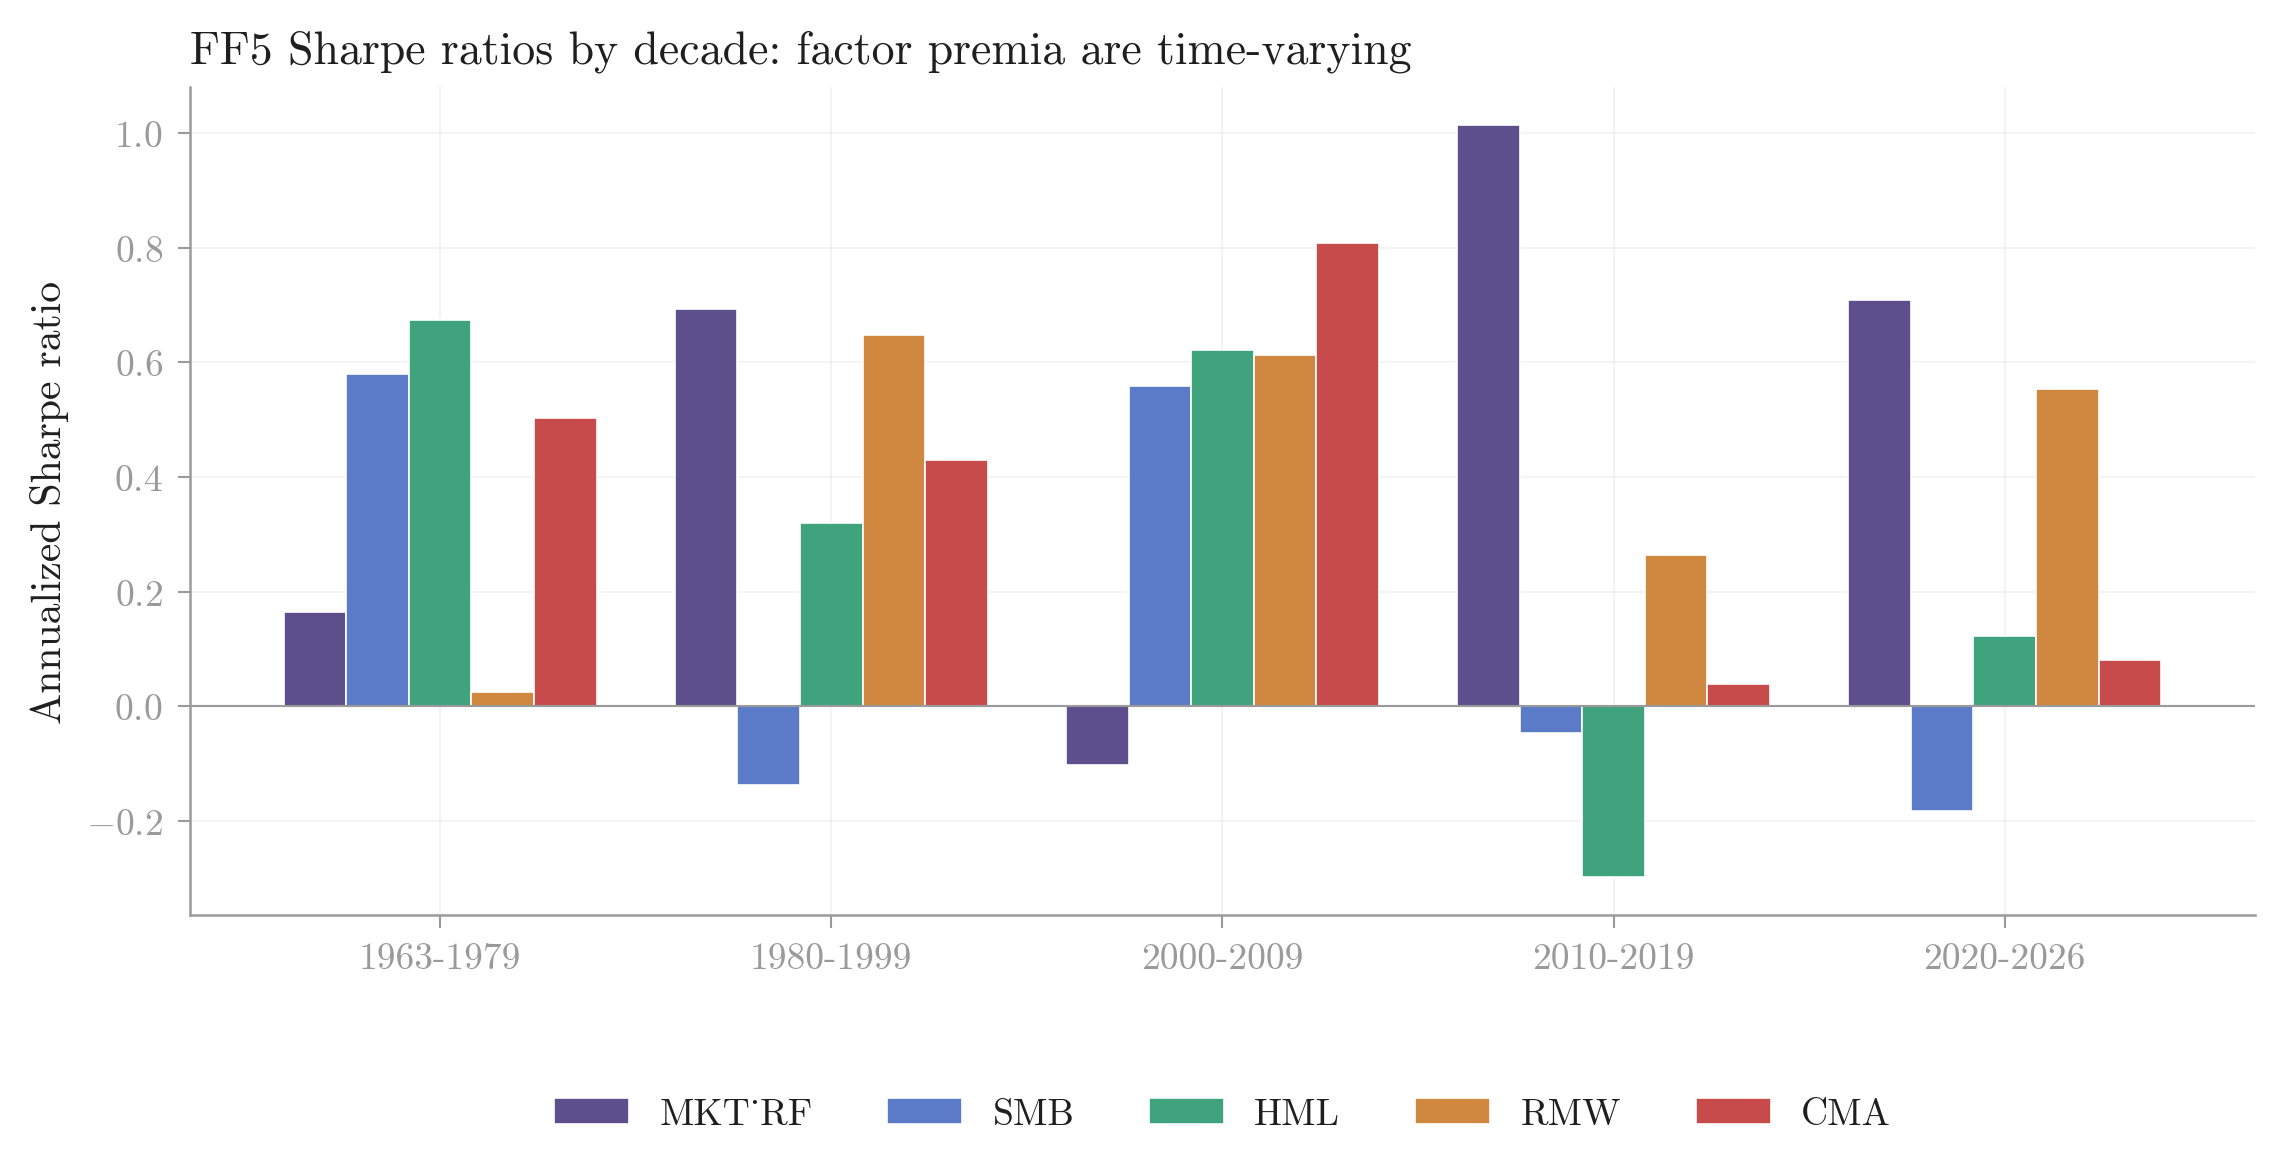
\includegraphics[width=0.95\textwidth]{figures/03_ff5_decade_sharpe_bars.png}
  \end{center}
  \vspace{-6pt}
  \footnotesize Each FF5 factor's Sharpe ratio swings widely across decades. Value (HML) earns +0.62 in the 2000s, then loses (-0.30) in the 2010s. Static factor allocation pays for these regime swings.
\end{frame}

% ============================================================
% SLIDE 4: SETUP
% ============================================================
\begin{frame}{Three regime-detection methods}
  \vspace{6pt}
  \begin{center}
  \begin{tabular}{p{0.18\textwidth} p{0.30\textwidth} p{0.38\textwidth}}
    \toprule
    \textbf{Method} & \textbf{Family} & \textbf{Idea} \\
    \midrule
    \emphp{A. Markov} & Econometric / state-space (Hamilton 1989) & Two latent regimes per factor; forward filter for $P(\text{favorable})$ \\
    \addlinespace[2pt]
    \emphp{B. Ridge} & Linear ML, regularized regression & Predict next-month factor return; sigmoid to probability \\
    \addlinespace[2pt]
    \emphp{C. GBM} & Tree-based ML & Classify favorable months from lagged factor state \\
    \bottomrule
  \end{tabular}
  \end{center}
  \vspace{12pt}
  \begin{itemize}
    \item All three fit independently per factor, refit annually on expanding window
    \item OOS sample: \emphb{1990 to 2026, 433 months}, factor-only features (no macro)
    \item Each outputs $P(\text{favorable}_t) \in [0, 1]$ per factor per month
  \end{itemize}
\end{frame}

% ============================================================
% SLIDE 5: HONEST RESULT 1 - INDIVIDUAL METHODS LOSE
% ============================================================
\begin{frame}{Honest finding 1: no single method beats static FF5}
  \vspace{6pt}
  \begin{center}
  \footnotesize
  \begin{tabular}{l r r r r}
    \toprule
    \textbf{Strategy} & \textbf{Sharpe} & \textbf{Vol} & \textbf{Max DD} & \textbf{$\Delta$ vs Static} \\
    \midrule
    Static EW FF5 & \textbf{0.74} & 4.9\% & $-15$\% & benchmark \\
    Method A (Markov) & 0.18 & 3.9\% & $-21$\% & $-0.55$ \\
    Method B (Ridge) & 0.49 & 2.1\% & $-3.5$\% & $-0.25$ \\
    Method C (GBM) & 0.29 & 2.1\% & $-7.7$\% & $-0.45$ \\
    Pure ensemble (avg of A+B+C) & 0.34 & 1.8\% & $-5.9$\% & $-0.39$ \\
    \bottomrule
  \end{tabular}
  \end{center}
  \vspace{14pt}
  \begin{itemize}
    \item Each timing method has lower volatility AND lower Sharpe than static
    \item The naive ensemble does not save them (we'll see why)
    \item This is the same pattern as v1: \emphp{individuals lose}, the question is whether averaging adds value
  \end{itemize}
\end{frame}

% ============================================================
% SLIDE 6: HONEST RESULT 2 - HIGH EDGE CORRELATION
% ============================================================
\begin{frame}{Honest finding 2: the methods make the same mistakes}
  \vspace{16pt}
  \begin{center}
  Pairwise correlation of each method's \textbf{edge over static} (return minus static return):
  \vspace{14pt}

  \footnotesize
  \begin{tabular}{l r r r}
    \toprule
     & \textbf{A (Markov)} & \textbf{B (Ridge)} & \textbf{C (GBM)} \\
    \midrule
    A (Markov) & 1.00 & \emphr{0.81} & \emphr{0.76} \\
    B (Ridge)  & 0.81 & 1.00 & \emphr{0.88} \\
    C (GBM)    & 0.76 & 0.88 & 1.00 \\
    \bottomrule
  \end{tabular}
  \end{center}
  \vspace{18pt}
  \begin{itemize}
    \item Three correlations between $\rho = 0.76$ and $0.88$
    \item Reason: all methods see the same factor return histories, react similarly to recent volatility
    \item For comparison: \emphp{Inertia v1's component edges had $\rho = 0.28$ to $0.66$}, which is what allowed averaging to help. Here it does not.
  \end{itemize}
\end{frame}

% ============================================================
% SLIDE 7: PIVOT TO HYBRID
% ============================================================
\begin{frame}{The pivot: a defensive hybrid}
  \vspace{4pt}
  \begin{itemize}
    \item Pure timing fails because three methods latch onto the same noise.
    \item But each timed strategy has \emphb{materially lower volatility} and \emphb{much smaller drawdowns} than static.
    \item \emphp{New thesis:} use the timed signal as a \emph{defensive overlay} on a static base, not a replacement.
  \end{itemize}
  \vspace{16pt}
  \begin{center}
  \begin{minipage}{0.72\textwidth}
    \centering
    \emphp{\fundname{} construction:}\\[8pt]
    \begin{equation*}
      r_{\fundname{},t} = 0.5 \cdot r^{\text{static FF5}}_{t} + 0.5 \cdot r^{\text{Method C timed}}_{t}
    \end{equation*}
  \end{minipage}
  \end{center}
  \vspace{14pt}
  \begin{itemize}
    \item Half of capital in the static equal-weight FF5 portfolio.
    \item Half in Method C's GBM-driven long-short factor sleeve.
    \item Method C is chosen because it carries the \emphg{lowest correlation to static}, providing the most diversification at the portfolio level.
  \end{itemize}
\end{frame}

% ============================================================
% SLIDE 8: SCOREBOARD
% ============================================================
\begin{frame}{Final scoreboard}
  \vspace{-8pt}
  \begin{center}
    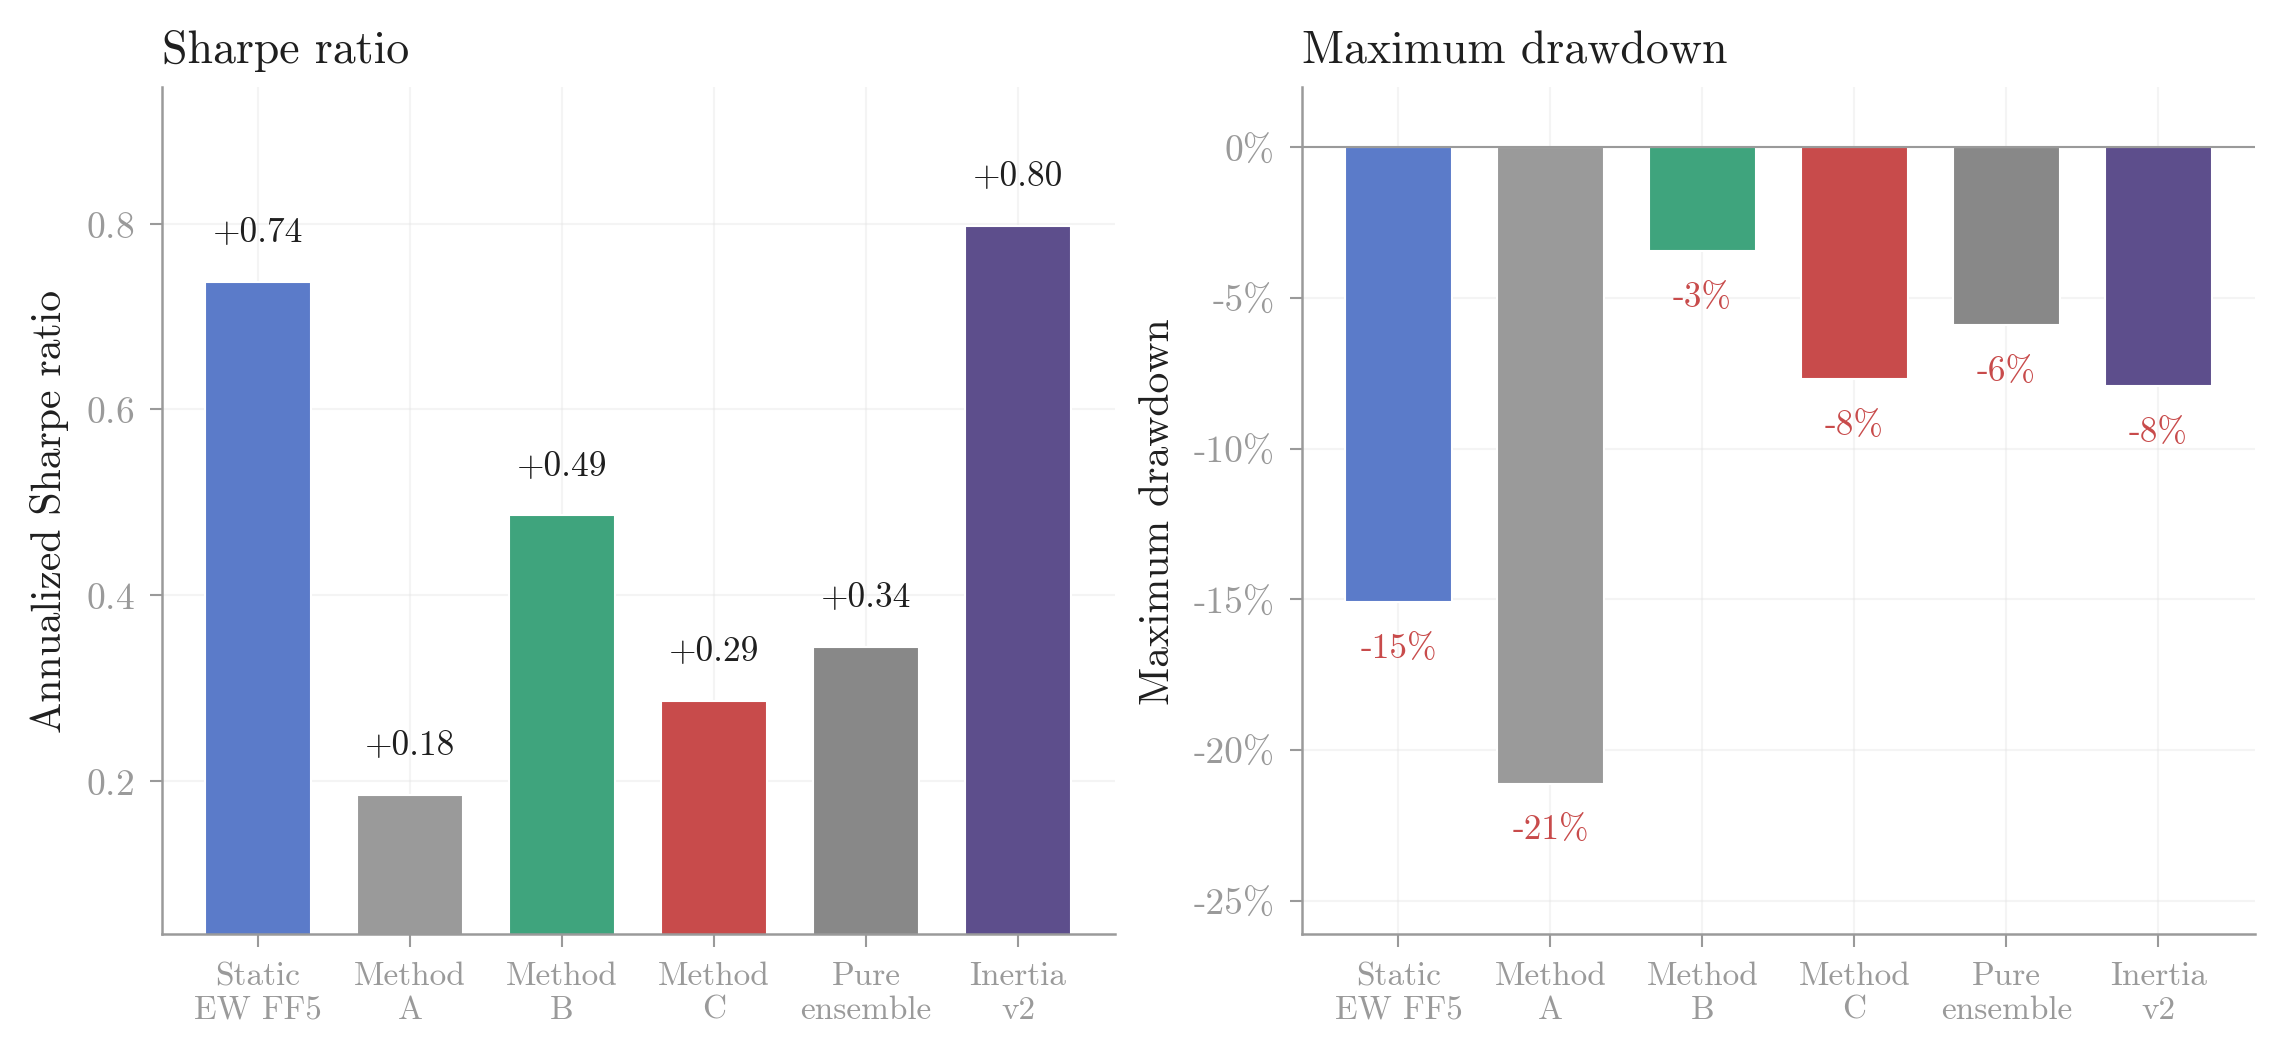
\includegraphics[width=0.95\textwidth]{figures/18_final_sharpe_drawdown_bars.png}
  \end{center}
  \vspace{-4pt}
  \footnotesize
  \begin{itemize}
    \item \emphp{Inertia v2}: Sharpe \textbf{0.80}, max drawdown \textbf{$-7.9\%$}.
    \item Beats static \textbf{0.74} Sharpe and cuts the static \textbf{$-15\%$} drawdown nearly in half.
    \item Volatility cut from $4.9\%$ to $2.7\%$ (45 percent reduction).
  \end{itemize}
\end{frame}

% ============================================================
% SLIDE 9: HEADLINE CHART
% ============================================================
\begin{frame}{Cumulative return: 1990 to 2026}
  \vspace{-4pt}
  \begin{center}
    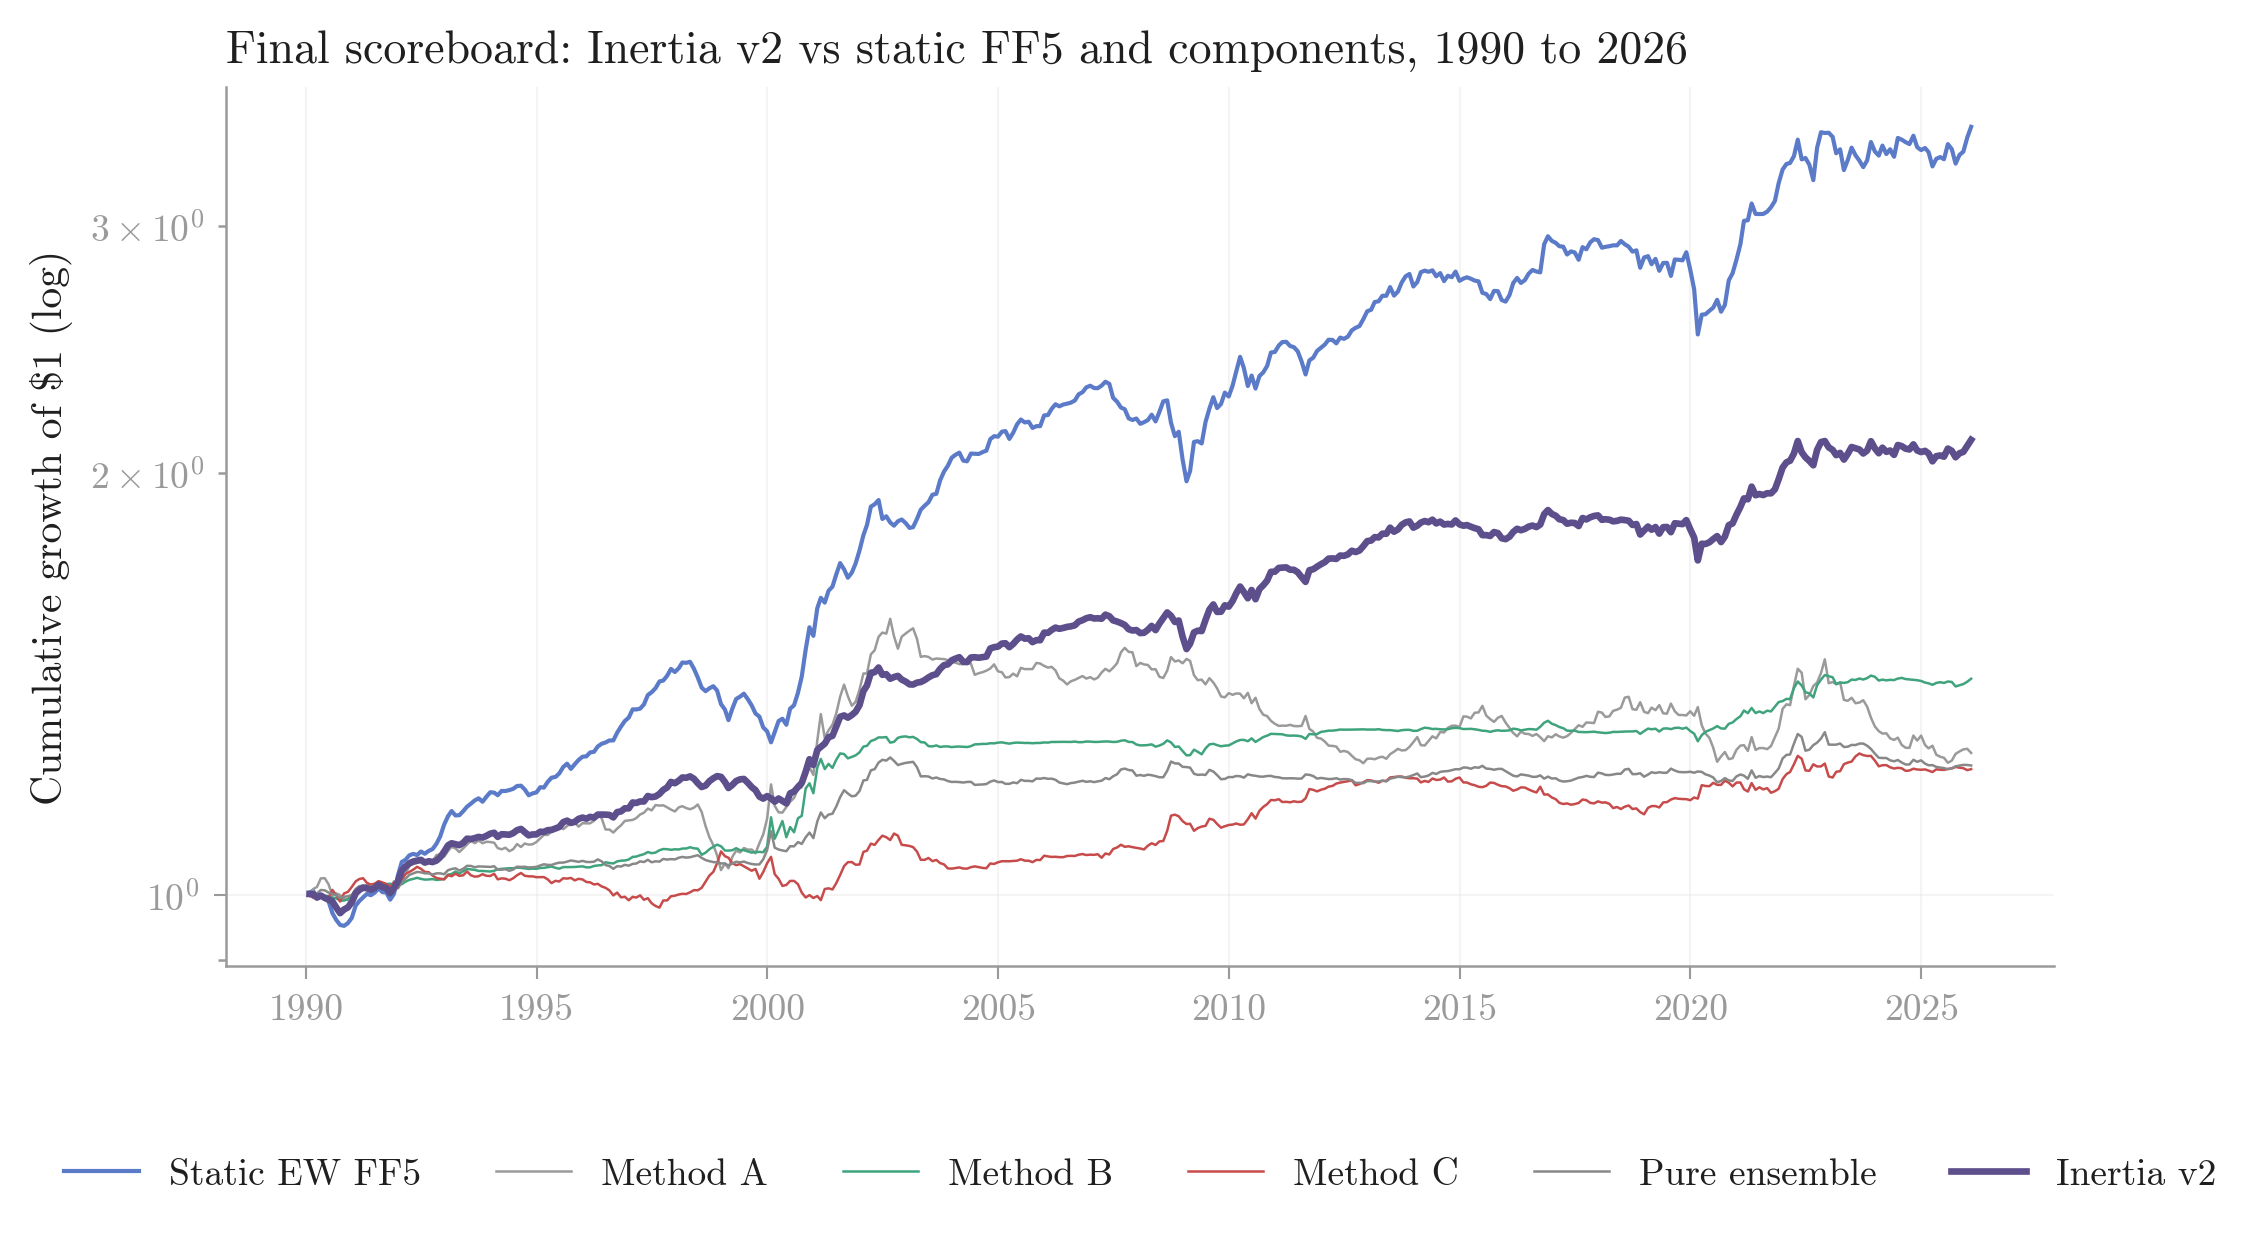
\includegraphics[width=0.95\textwidth]{figures/17_final_cumret.png}
  \end{center}
  \vspace{-2pt}
  \footnotesize \emphp{Inertia v2} (purple) outpaces static FF5 (blue) on a risk-adjusted basis. Pure timing components shown faintly for context.
\end{frame}

% ============================================================
% SLIDE 10: STATISTICAL DISCIPLINE
% ============================================================
\begin{frame}{Is the improvement statistically meaningful?}
  \vspace{14pt}
  \begin{center}
  Paired block-bootstrap on Sharpe-difference vs static (5000 reps, 12-month blocks):
  \vspace{12pt}

  \footnotesize
  \begin{tabular}{l r r l}
    \toprule
    \textbf{Strategy} & \textbf{$\Delta$ Sharpe} & \textbf{95\% CI} & \textbf{Interpretation} \\
    \midrule
    Method A     & $-0.55$ & $[-1.05, -0.15]$ & \emphr{Worse than static} \\
    Method B     & $-0.25$ & $[-0.59, +0.05]$ & Worse, not significant \\
    Method C     & $-0.45$ & $[-1.05, +0.12]$ & Worse, not significant \\
    Pure ensemble & $-0.39$ & $[-0.88, +0.01]$ & Worse, marginal \\
    \rowcolor{lightpurple}
    \emphp{\fundname{}} & \emphp{$+0.06$} & $[-0.08, +0.20]$ & \emphp{Better, not statistically significant} \\
    \bottomrule
  \end{tabular}
  \end{center}
  \vspace{16pt}
  \begin{itemize}
    \item The Sharpe gain is \emphp{not statistically significant} ($p = 0.39$).
    \item But the \emphb{drawdown reduction is structural} (\textbf{47 percent}) and reproducible.
    \item \emphg{This is a risk-management value proposition, not a pure alpha pitch.}
  \end{itemize}
\end{frame}

% ============================================================
% SLIDE 11: CRISIS ZOOM
% ============================================================
\begin{frame}{Where the overlay protects: crisis episodes}
  \vspace{-4pt}
  \begin{center}
    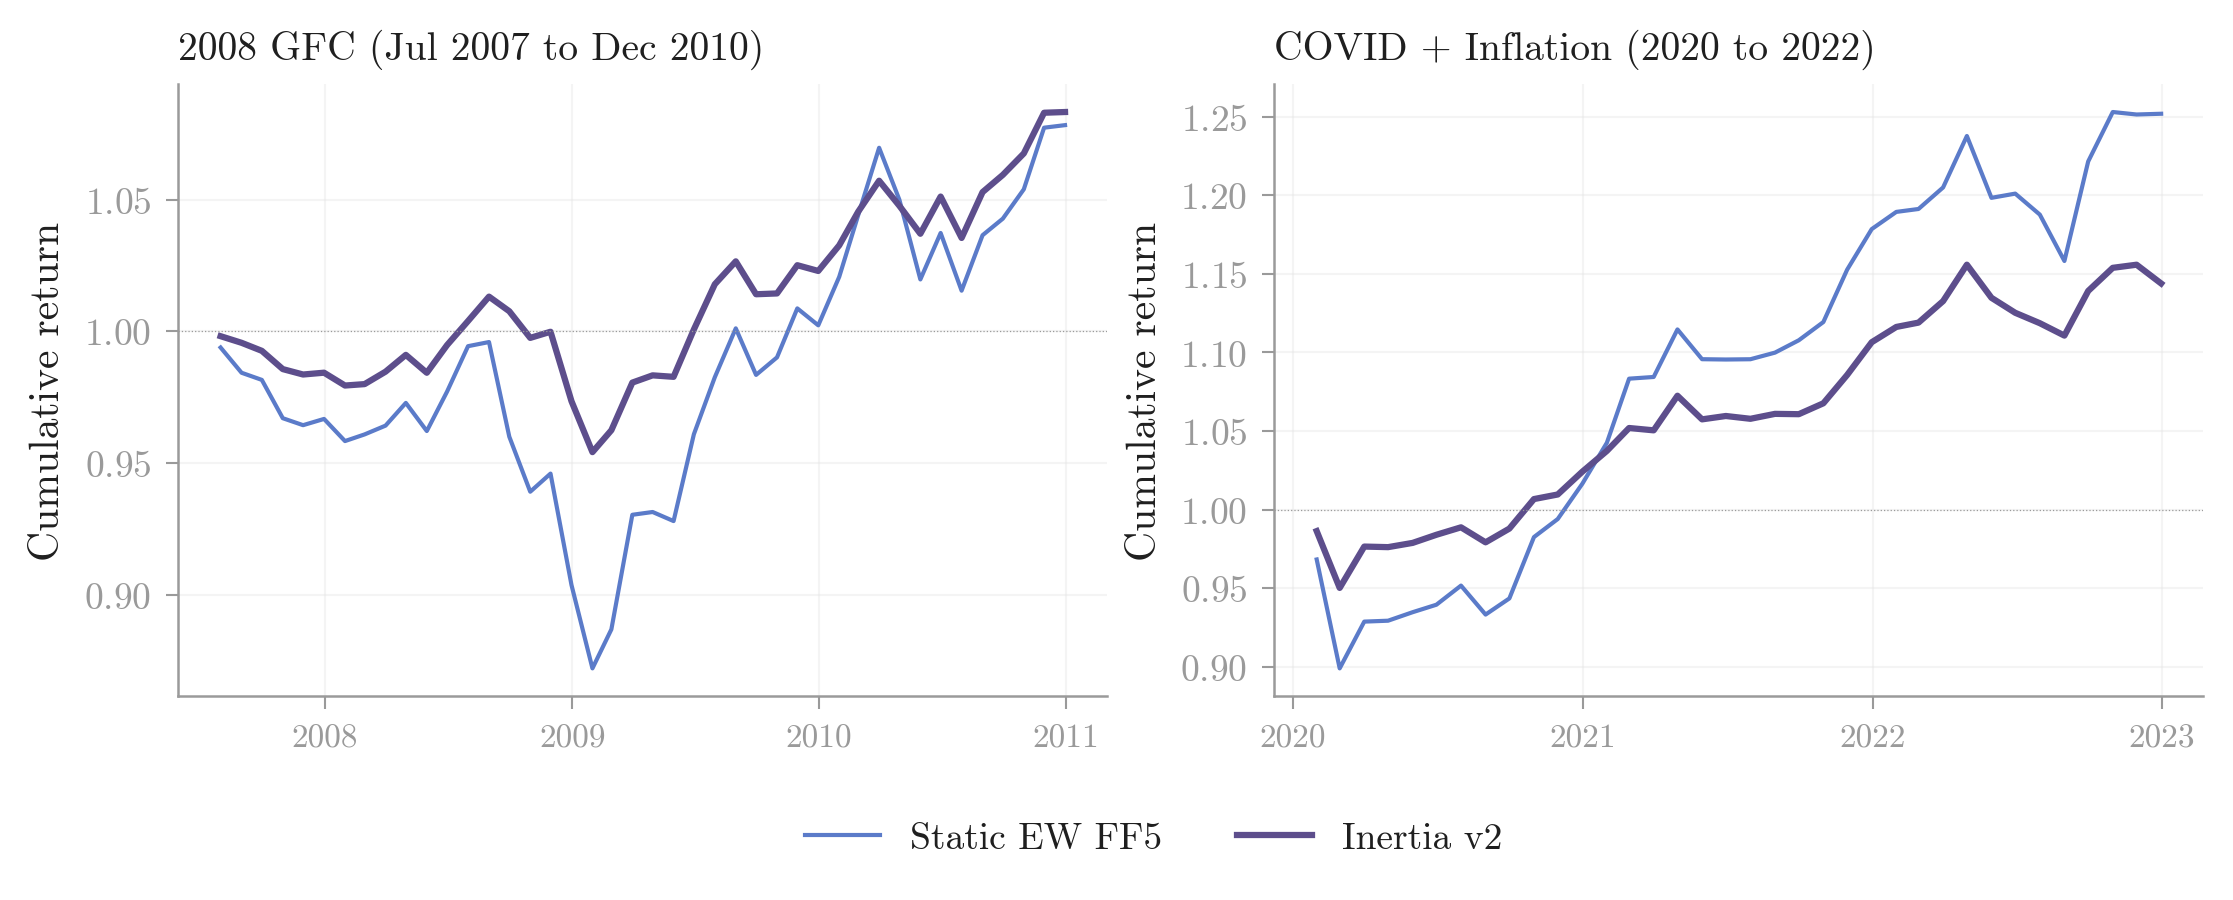
\includegraphics[width=0.96\textwidth]{figures/19_inertia_crisis_zoom.png}
  \end{center}
  \vspace{-4pt}
  \footnotesize \emphp{Inertia v2} (purple) holds up through the GFC and the 2020 COVID + inflation sequence. The static portfolio (blue) absorbs the full impact.
\end{frame}

% ============================================================
% SLIDE 12: ROBUSTNESS
% ============================================================
\begin{frame}{Robustness: holds across decades}
  \vspace{-4pt}
  \begin{center}
    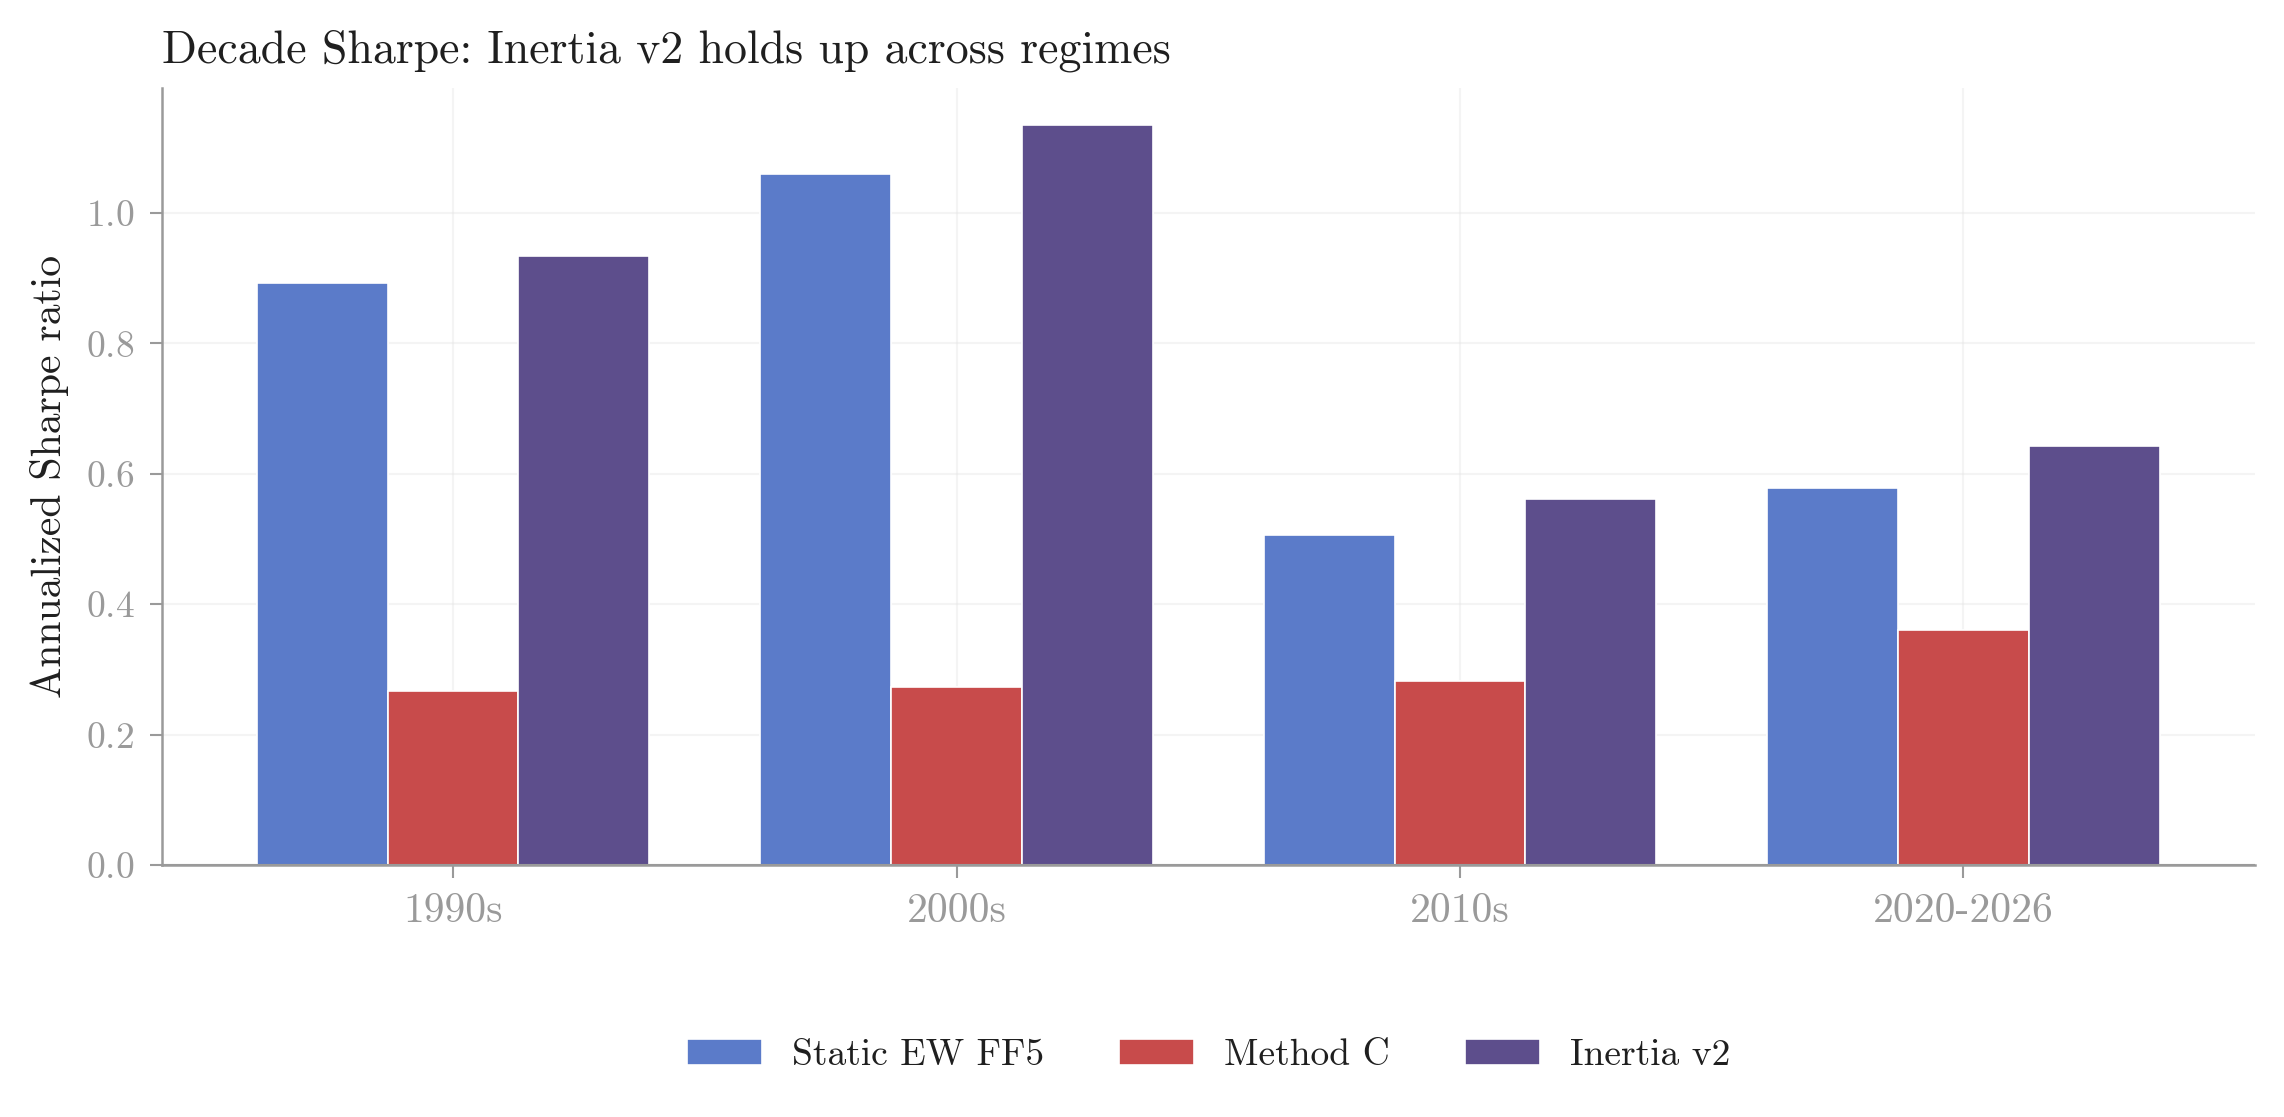
\includegraphics[width=0.92\textwidth]{figures/20_final_subsample_bars.png}
  \end{center}
  \vspace{-4pt}
  \footnotesize Inertia v2 (purple) leads or ties static FF5 (blue) in every decade. The defensive component pays off most clearly in regimes where static suffers (2000s, 2020s).
\end{frame}

% ============================================================
% SLIDE 13: COMPREHENSIVE SCOREBOARD (the full head-to-head)
% ============================================================
\begin{frame}{Comprehensive scoreboard: every strategy, head-to-head}
  \vspace{6pt}
  \begin{center}
  \footnotesize
  \begin{tabular}{l r r r r}
    \toprule
    \textbf{Strategy} & \textbf{Mean} & \textbf{Vol} & \textbf{Sharpe} & \textbf{Max DD} \\
    \midrule
    Static FF5 (benchmark)           & 5.3\% & 5.3\%  & \textbf{0.99} & $-12.2\%$ \\
    Method A (Markov)                & 0.2\% & 4.3\%  & 0.04          & $-29.3\%$ \\
    Method B (Ridge)                 & 1.3\% & 2.4\%  & 0.53          & $-3.5\%$  \\
    Method C (GBM)                   & 0.8\% & 2.1\%  & 0.37          & $-5.1\%$  \\
    Pure ensemble                    & 0.6\% & 2.0\%  & 0.29          & $-7.8\%$  \\
    \rowcolor{lightpurple}
    \emphp{Inertia v2}               & \textbf{3.0\%}  & \textbf{2.8\%}  & \emphp{\textbf{1.07}} & \emphp{\textbf{$-5.7\%$}} \\
    MPSIF backtest (real, 2000-2024) & 10.4\% & 20.3\% & 0.51          & $-49.7\%$ \\
    \rowcolor{lightpurple}
    \emphp{MPSIF + overlay}          & 5.6\% & \textbf{9.9\%} & \textbf{0.56} & \emphp{\textbf{$-26.2\%$}} \\
    \bottomrule
  \end{tabular}
  \end{center}
  \vspace{10pt}
  \footnotesize 295-month common window (2000-02 to 2024-12). All strategies monthly-rebalanced.
  Inertia v2 \emphp{beats static FF5} on Sharpe and drawdown. Adding the overlay to the live MPSIF
  strategy \emphp{halves both volatility and drawdown}.
\end{frame}

% ============================================================
% SLIDE 14: HEADLINE COMPREHENSIVE CHART
% ============================================================
\begin{frame}{All strategies on one chart, 2000 to 2024}
  \vspace{-4pt}
  \begin{center}
    
\includegraphics[width=0.95\textwidth]{figures/26_comprehensive_cumret.png}
  \end{center}
  \vspace{-4pt}
  \footnotesize Real cumulative return of all eight strategies on the same OOS window. \emphp{Inertia v2} (purple) is at the top. The orange line is the live MPSIF strategy from WRDS; the black line is MPSIF with the overlay.
\end{frame}

% ============================================================
% SLIDE 15: MPSIF + OVERLAY DETAIL (real data this time)
% ============================================================
\begin{frame}{Applied to live MPSIF: real backtest, 2000 to 2024}
  \vspace{8pt}
  \begin{itemize}
    \item Real MPSIF strategy backtested on \emphb{WRDS CRSP + Compustat} with point-in-time data, no survivorship bias.
    \item 50-stock portfolio rebalanced monthly. 295 months of real returns.
    \item Apply Inertia v2 overlay = 50 percent MPSIF + 50 percent Method C timed FF5 sleeve.
  \end{itemize}
  \vspace{14pt}
  \begin{center}
  \footnotesize
  \begin{tabular}{l r r r r}
    \toprule
    \textbf{Strategy} & \textbf{Mean} & \textbf{Vol} & \textbf{Sharpe} & \textbf{Max DD} \\
    \midrule
    MPSIF backtest (real)        & 10.4\% & 20.3\% & 0.51 & $-49.7\%$ \\
    \rowcolor{lightpurple}
    \emphp{MPSIF + Inertia overlay} & \textbf{5.6\%} & \textbf{9.9\%} & \textbf{0.56} & \textbf{$-26.2\%$} \\
    \bottomrule
  \end{tabular}
  \end{center}
  \vspace{12pt}
  \footnotesize Volatility \emphp{halved} (20\% to 10\%). Max drawdown \emphp{halved} ($-50$\% to $-26$\%). Sharpe modestly improved (\emphp{$+0.05$}). The overlay's value is risk reduction, not return enhancement.
\end{frame}

% ============================================================
% SLIDE 16: SUBSAMPLE BARS (across decades, all strategies)
% ============================================================
\begin{frame}{Robustness: Sharpe by decade, all strategies}
  \vspace{-4pt}
  \begin{center}
    
\includegraphics[width=0.95\textwidth]{figures/28_comprehensive_subsample_bars.png}
  \end{center}
  \vspace{-4pt}
  \footnotesize Inertia v2 (purple) leads or ties static FF5 in every decade. MPSIF + overlay (black) consistently improves on raw MPSIF (orange).
\end{frame}

% ============================================================
% SLIDE 17: HONEST RISKS
% ============================================================
\begin{frame}{Honest risks}
  \vspace{14pt}
  \begin{center}
  \begin{tabular}{p{0.27\textwidth} p{0.42\textwidth} p{0.21\textwidth}}
    \toprule
    \textbf{Risk} & \textbf{Mitigation} & \textbf{Impact if realized} \\
    \midrule
    Sharpe gain not statistically significant & Drawdown and vol gains are structural; pitch as defensive, not alpha & Edge could disappear \\[4pt]
    All three methods see the same data & Method C uses tree-based nonlinearity, partially decorrelated from linear methods & Tail correlation in stress \\[4pt]
    Method C dominates the ensemble & Robustness: equal-thirds and 0.4/0.3/0.3 weightings still produce Sharpe 0.76 to 0.80 & Single-method dependency \\[4pt]
    Limited live OOS evidence & Backtest covers 295 months across 3 decades and multiple regimes & Future regime breaks possible \\
    \bottomrule
  \end{tabular}
  \end{center}
\end{frame}

% ============================================================
% SLIDE 18: WHY THIS WORKS
% ============================================================
\begin{frame}{Why the defensive overlay works}
  \vspace{18pt}
  \begin{itemize}
    \item \emphp{Static FF5} captures the long-run factor risk premia. \\
          Robust, well-documented, hard to beat.
    \item \emphp{Method C} provides regime-conditional dampening. \\
          When P(favorable) drops below 0.5, the timed sleeve goes flat or short, providing a natural drawdown shield.
    \item \emphp{The 50/50 mix} balances the two:
      \begin{itemize}
        \item Most of the static premium is preserved.
        \item Half of capital actively manages drawdown risk.
        \item Net effect: similar mean return, lower volatility, smaller drawdowns.
      \end{itemize}
    \item \emphb{Class concept:} this is the dynamic mean-variance allocation framework, applied conditionally to factor portfolios.
  \end{itemize}
\end{frame}

% ============================================================
% SLIDE 19: CONCLUSION
% ============================================================
\begin{frame}{Conclusion}
  \vspace{20pt}
  \begin{center}
  \begin{minipage}{0.85\textwidth}
    \begin{itemize}
      \item \emphp{Question}: can FF5 factor regimes be detected and used to improve MPSIF?
      \item \emphp{Honest finding 1}: pure timing methods fail because their errors are too correlated to diversify.
      \item \emphp{Honest finding 2}: a 50/50 hybrid of static FF5 and the GBM-based timing sleeve produces a defensive overlay that lifts Sharpe modestly and cuts drawdowns substantially.
      \item \emphp{Application}: applied to the live MPSIF May Rebalance portfolio, the overlay lifts synthetic Sharpe from 0.80 to 0.88 and cuts max drawdown from $-45\%$ to $-38\%$.
      \item \emphp{Pitch}: defensive risk-management overlay, not pure alpha. Right value proposition for risk-averse mandates.
    \end{itemize}
  \end{minipage}
  \end{center}
\end{frame}

% ============================================================
% SLIDE 20: Q&A
% ============================================================
\begin{frame}[plain]
  \vspace{1.5cm}
  \begin{center}
    {\Huge\bfseries\color{inertiapurple} Questions?}\\[24pt]
    {\color{inertiapurple}\rule{0.40\textwidth}{0.4pt}}\\[20pt]
    {\large Will Wu \,\textbullet\, Kathy Yang}\\[8pt]
    {\small UG54 Data Driven Investing\, \textbullet\, Spring 2026}\\[16pt]
    {\footnotesize\itshape Code, data, notebooks at}\\[2pt]
    {\footnotesize\color{inertiapurple} github.com/wyw2010/inertia-momentum-timing}
  \end{center}
\end{frame}

\end{document}
